
\subsection{Modalities}
The three chosen modes, visual, auditory, and visual-auditory combined, are chosen for testing. Feedback from each of these different modalities has been shown to improve task performance for small tasks~\cite{chi_oussama_tap_the_shapetones}. Combining modalities are essential for user interaction enabling systems to be highly flexible and accessible to varying ages~\cite{article_user_centred_multimodal_reminders}. Giving people a choice of mode to interact with gives people a highly configurable, non-disruptive system that provides alternative ways of interaction~\cite{article_designing_multimodal_reminders_for_home, multi_modal_reminders_less_disruptive}. Technology to support behaviour change should be non-disruptive to encourage usage. Habit rewards should not be annoying as positive reinforcement should be a satisfactory experience. Research into \textit{visual}, \textit{auditory} and \textit{visual-auditory} feedback was identified to understand how they impact behaviour to see how habit formation is impacted.

\begin{figure}[H]
  \centering
  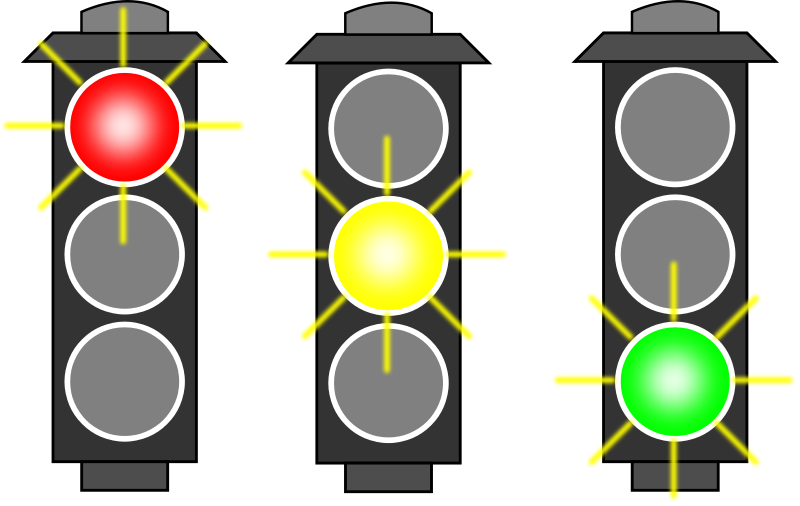
\includegraphics[width=2.6in]{../resources/visual.png}
  \hspace{10px}
  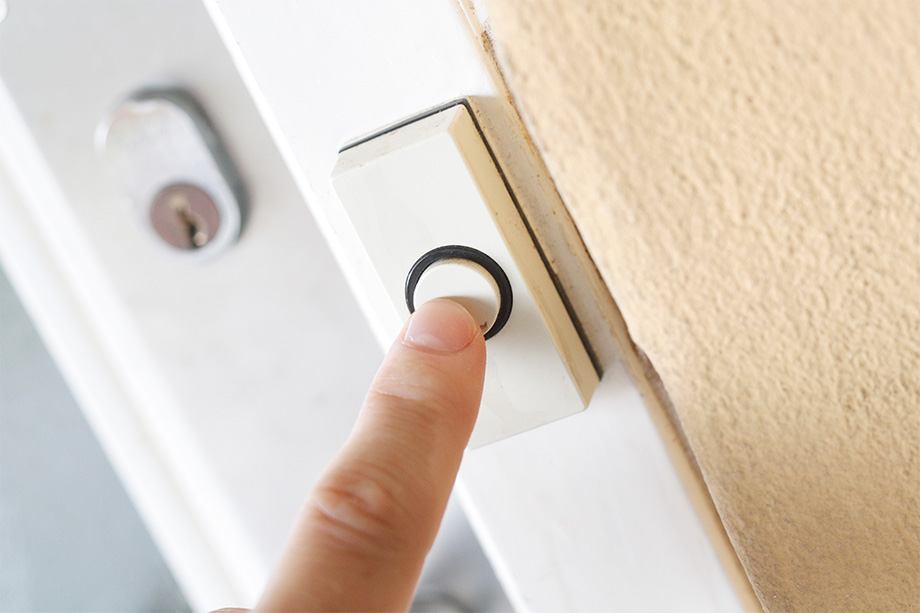
\includegraphics[width=2.6in]{../resources/audio.png}
  \caption{An example of visual (traffic light) and auditory (doorbell) feedback.}
  \label{fig:visual_audio}
\end{figure}

\subsubsection{Visual}
Visual feedback can encourage task performance consistency as demonstrated in one study by Matthew Lee et al.~\cite{article_realtime_feedback_improving_medication_taking} where they constructed a device that gave constant visual feedback for patients taking medication. They found that visual feedback improved consistency of the habit and increased the rate of self-efficacy. But when the device was removed, their performance dropped (as measured after a 2-month period). This suggests that users did integrate the visual feedback display cue with their routines, but they also became dependant on the technology and the visual feedback did not build habit strength. Users should instead build these cues outside of the system, with another routine to build habit automaticity and allowing for permanent behaviour change after the system is removed.

\subsubsection{Auditory}
There is a need to use sound when designing for behaviour change technology, especially with a varied target market~\cite{article_designing_for_health_behaviour_change_hci}. For example, combing different sounds for different actions to suit different users~\cite{article_movipill_improving_medication_elders}. Using auditory as a method of delivery has shown to improve task success~\cite{auditory_notifications_increase_delivery_success}, but little work has shown how it impacts habit performance.

\subsubsection{Visual-Auditory}
Several studies show that combining audio with visual as feedback after the completion of a simple task, can be successful e.g.~\cite{benefits_of_audio_visual_1, benefits_of_audio_visual_2}. A meta-analysis of 43 multi-modal studies~\cite{comparing_modalities_effects_of_visual_auditory} revealed that it was the most effective to increase performance, when a single task is being performed and when compared with visual or auditory feedback alone. Additional research shows this combination of visual and auditory sensory channels has been shown to increase performance with complex tasks~\cite{chi_oussama_tap_the_shapetones}. However, care needs to be taken when adding an extra modality as this study showed that '\textit{visual feedback improved task performance, but sacrificed task quality}'~\cite{comparing_modalities_effects_of_visual_auditory}. In addition, while all modalities contribute to perceptual experience, one sense can override another if the sensory channel mediates less ambiguous information than the other~\cite{one_mode_override_another}. Therefore it will be useful to compare the success of the task with the other modes. Using a combination of modalities for interaction gives a means of communication to people with varying levels of sensory awareness. A choice of mode when designing for interaction~\cite{article_user_centred_multimodal_reminders} is important, but system consistency is necessary.


Finally, the majority of electronic activity monitors have behaviour change techniques and these monitors present a medium which behaviour change interventions could occur. By using tactile vibration integrated into a wearable device. A survey on activity monitors~\cite{article_wearable_good} ranked Fitbit (\url{www.fitbit.com}) devices as good vehicles for behaviour change techniques. Therefore, the Fibit, would be a good primary platform for integrating vibration for rewards. However, due to technical limitations, as discussed in Section \ref{limitations_and_future_work}, we are unable to implement them.


% % Old version
% Habit formation research~\cite{article_understanding_use_contextual_cues_design_impl} shows how different contextual cues better support behaviour change, compared with a single mode.
% If we combine this with research~\cite{article_natural_cross_modal_mappings} into crossmodal interaction,
% i.e. the process of signals we receive through a single sense affecting how we process information perceived through a different sense.
% We can map habit rewards across different modalities, enabling us to present users with the same reward type from a different modality.
% This allows us to test the different types of modalities and how they effect behaviour change.
% The next section discusses methods of interaction in practice.

% \subsection{Why Interaction from Different Modalities}
% `Multi-modal systems are required for user interaction'~\cite{article_user_centred_multimodal_reminders} states research into comparing unimodal reminders systems with multimodal.
% They suggests a need for `highly flexible and contextualised multimodal and multi-device reminder systems'~\cite{article_user_centred_multimodal_reminders}.
% Although this study focused on the elderly, so the need to multiple modalities was important because some peoples sensory modalities decline with age,
% this principle still holds true for general case reminder systems. The study presents design guidelines for reminder systems.
% These are mainly focused on users needing a choice of modalities for interacting with users, as users want a highly configurable system.
% These aspects are implemented into our project and adapted for delivering rewards.\newline
% \newline
% Research into designing reminder systems for the home that interact with users in different modalities, states that
% `Good reminder systems should use different modalities, because they provide alternative ways to interact with a user'~\cite{article_designing_multimodal_reminders_for_home}.
% Using different modalities for interaction increases the likelihood that the information users are receiving are more pleasant to them,
% and decreases the chance the interaction will be disruptive or annoying~\cite{article_designing_multimodal_reminders_for_home}.
% Habit rewards should not be annoying, they should give users a feeling of satisfaction, therefore reducing the chance of disruption is another justification for using multiple modalities.


% \subsection{Habit Rewards}

% Why habit rewards?


% \subsection{Modality Types}
% Next we look at literature discussing the three main modality types and how they change peoples behaviour.

% \subsubsection*{Visual}
% One study looked at improving habit consistency for how often patients took medication,
% by using a visual display device that gave constant feedback~\cite{article_realtime_feedback_improving_medication_taking}.
% They found that this feedback improved consistency of the habit and increasing rating of self-efficacy.
% But when the device was removed, their performance dropped (from a 2-month follow up study), because users integrated the feedback display with their routines.
% This habit-forming system used visual feedback to encourage consistency, however, this system shouldn't integrate visual cues into the system, otherwise users become dependent on the technology.
% Users should instead build these cues outside of the system to build performance longevity after removing the system.

% \subsubsection*{Auditory}
% Another key paper, discussed their need for different modalities when designing for the elderly~\cite{article_movipill_improving_medication_elders},
% combing different sounds with high visual contrast to suit their needs, given deteriorating senses due to age.
% The study showed that using different modalities for interaction gives a means of communication to people with varying levels of sense ability.
% But studies have also shown people need a choice of mode when designing for interaction~\cite{article_user_centred_multimodal_reminders},
% and thus the design requirements produced from this study can be applied to general applications that use multiple modalities, such as this project.
% The design guidelines discuss the need for interaction consistency, such as using similar audio interaction.
% Therefore visual and auditory rewards are mapped identifying a pattern across the modalities.

% Additional reserach, supports the use of tactile cues to improve information transfer~\cite{tactile_improves_info_transfer}

% \subsection{Reward Types}
% Rewards are delivered from each modality, with the content based on requirements created in (TODO reference chapter 2).
% Visual rewards present the user with a gif to give them satisfaction after completing the action and auditory rewards provide a similar result but via the auditory mode.
% The next section discusses design recommendations for delivery methods for these rewards.

% \subsection{Pairing Reward types}

% Talk about how you can match Visual with sound, and breifly vibration.
% Disucssion about types of rewards.

% A Modal, setting the same frequency for sound and vibration, look into how mapping patterns TODO.

% Experiment with gif to audio to vibration
